\documentclass[12pt]{article}


\usepackage{amssymb}
\usepackage{amsmath}
\usepackage{fullpage}
\usepackage{epsfig}
\usepackage{epstopdf, xcolor, hyperref}
\everymath{\displaystyle}
\usepackage{enumerate}

\newif\ifans

\anstrue

\begin{document}

\begin{center}
\underline{\LARGE{Jacobian \& Change of Variables}}
\end{center}

\noindent SUGGESTED REFERENCE MATERIAL:

\bigskip

\noindent As you work through the problems listed below, you should reference Chapter 14.7 of the recommended textbook (or the equivalent chapter in your alternative textbook/online resource) and your lecture notes.

\bigskip

\noindent EXPECTED SKILLS:

\begin{itemize}

\item Be able to use the change of variable formulas (14.7.2 and 14.7.4) for converting an integral from rectangular coordinates to another coordinate system by changing the integrand, the region of integration, and including the Jacobian factor.

\end{itemize}

\noindent PRACTICE PROBLEMS:

\medskip

\begin{enumerate}

\item For each of the following, sketch the image of the region under the given transformation.

\begin{enumerate}

\item $R$ is the region shown below and the transformation is: $x=r\cos{\theta}$, $y=r\sin{\theta}$, with $r \geq 0$ and $0 \leq \theta \leq 2\pi$.

\begin{center}
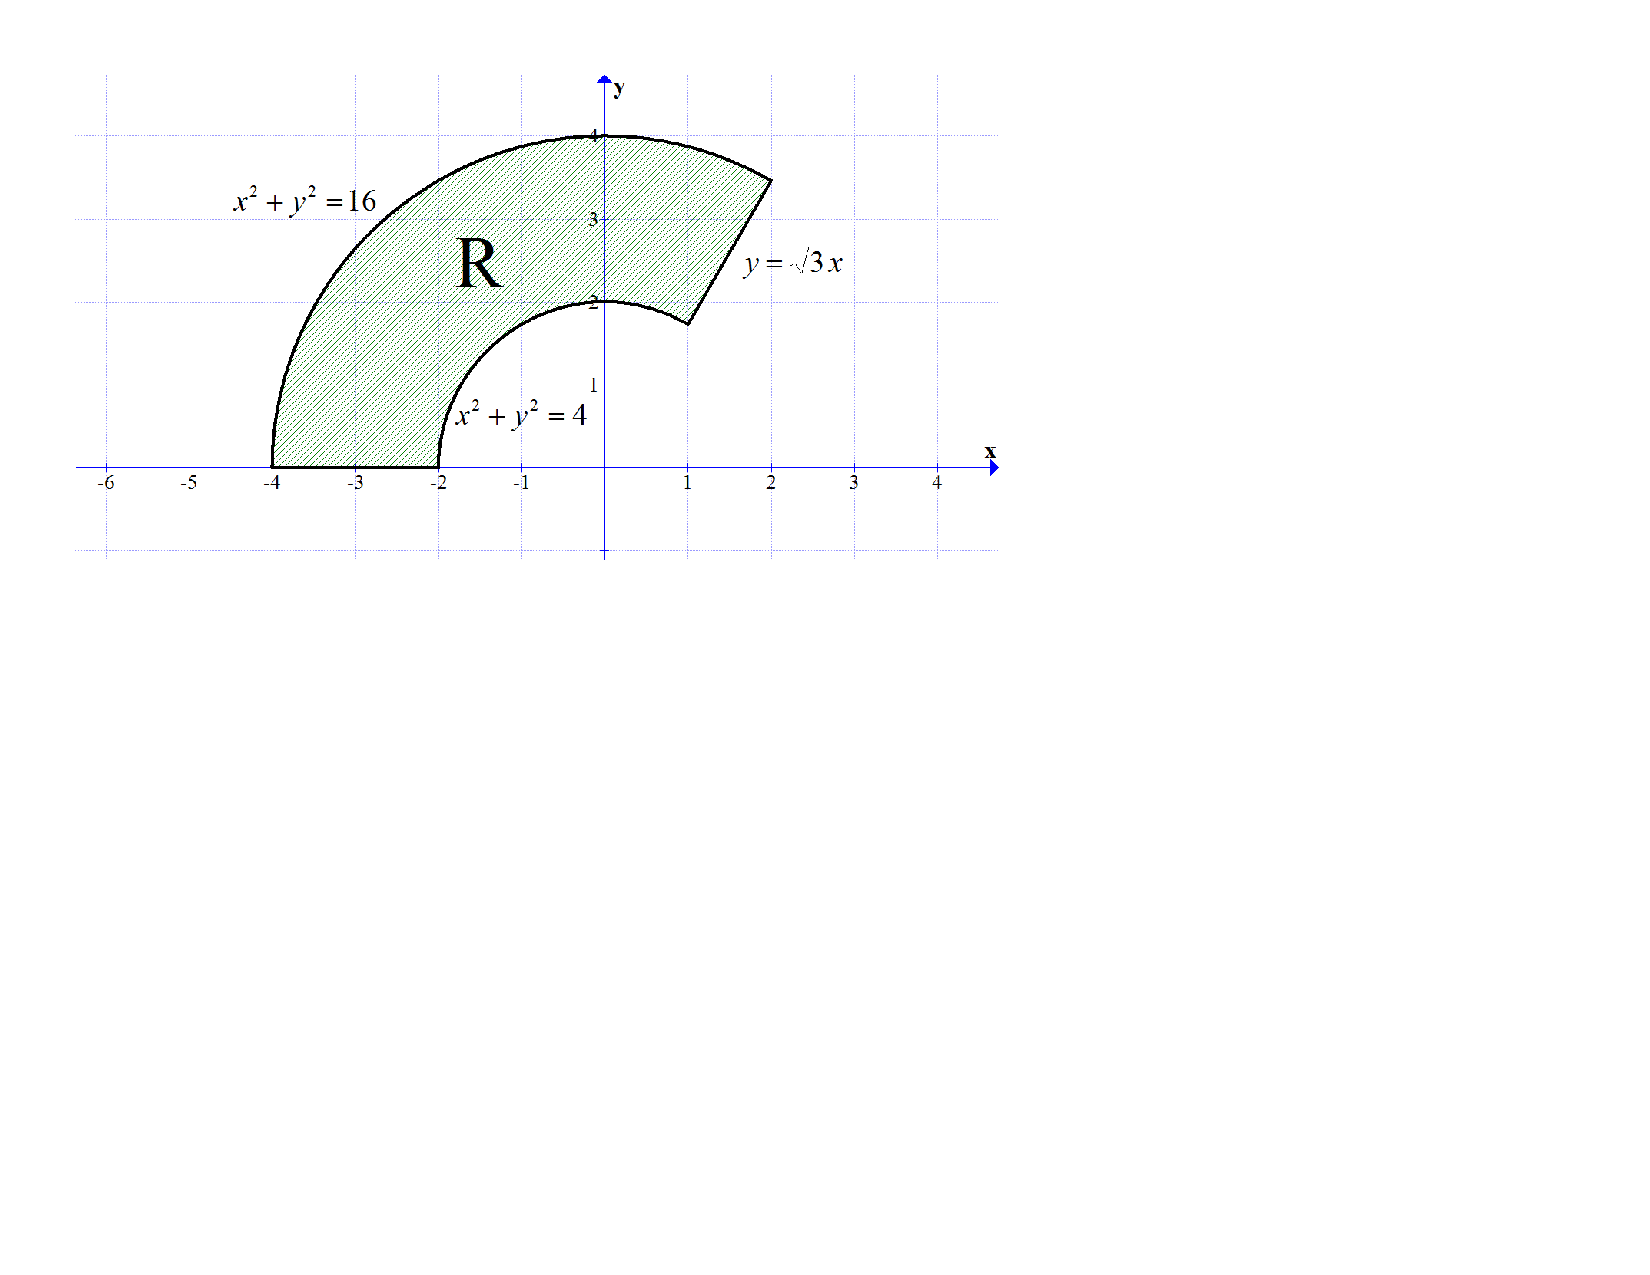
\includegraphics[scale=0.6]{region1.pdf}
\end{center}

\ifans{\fbox{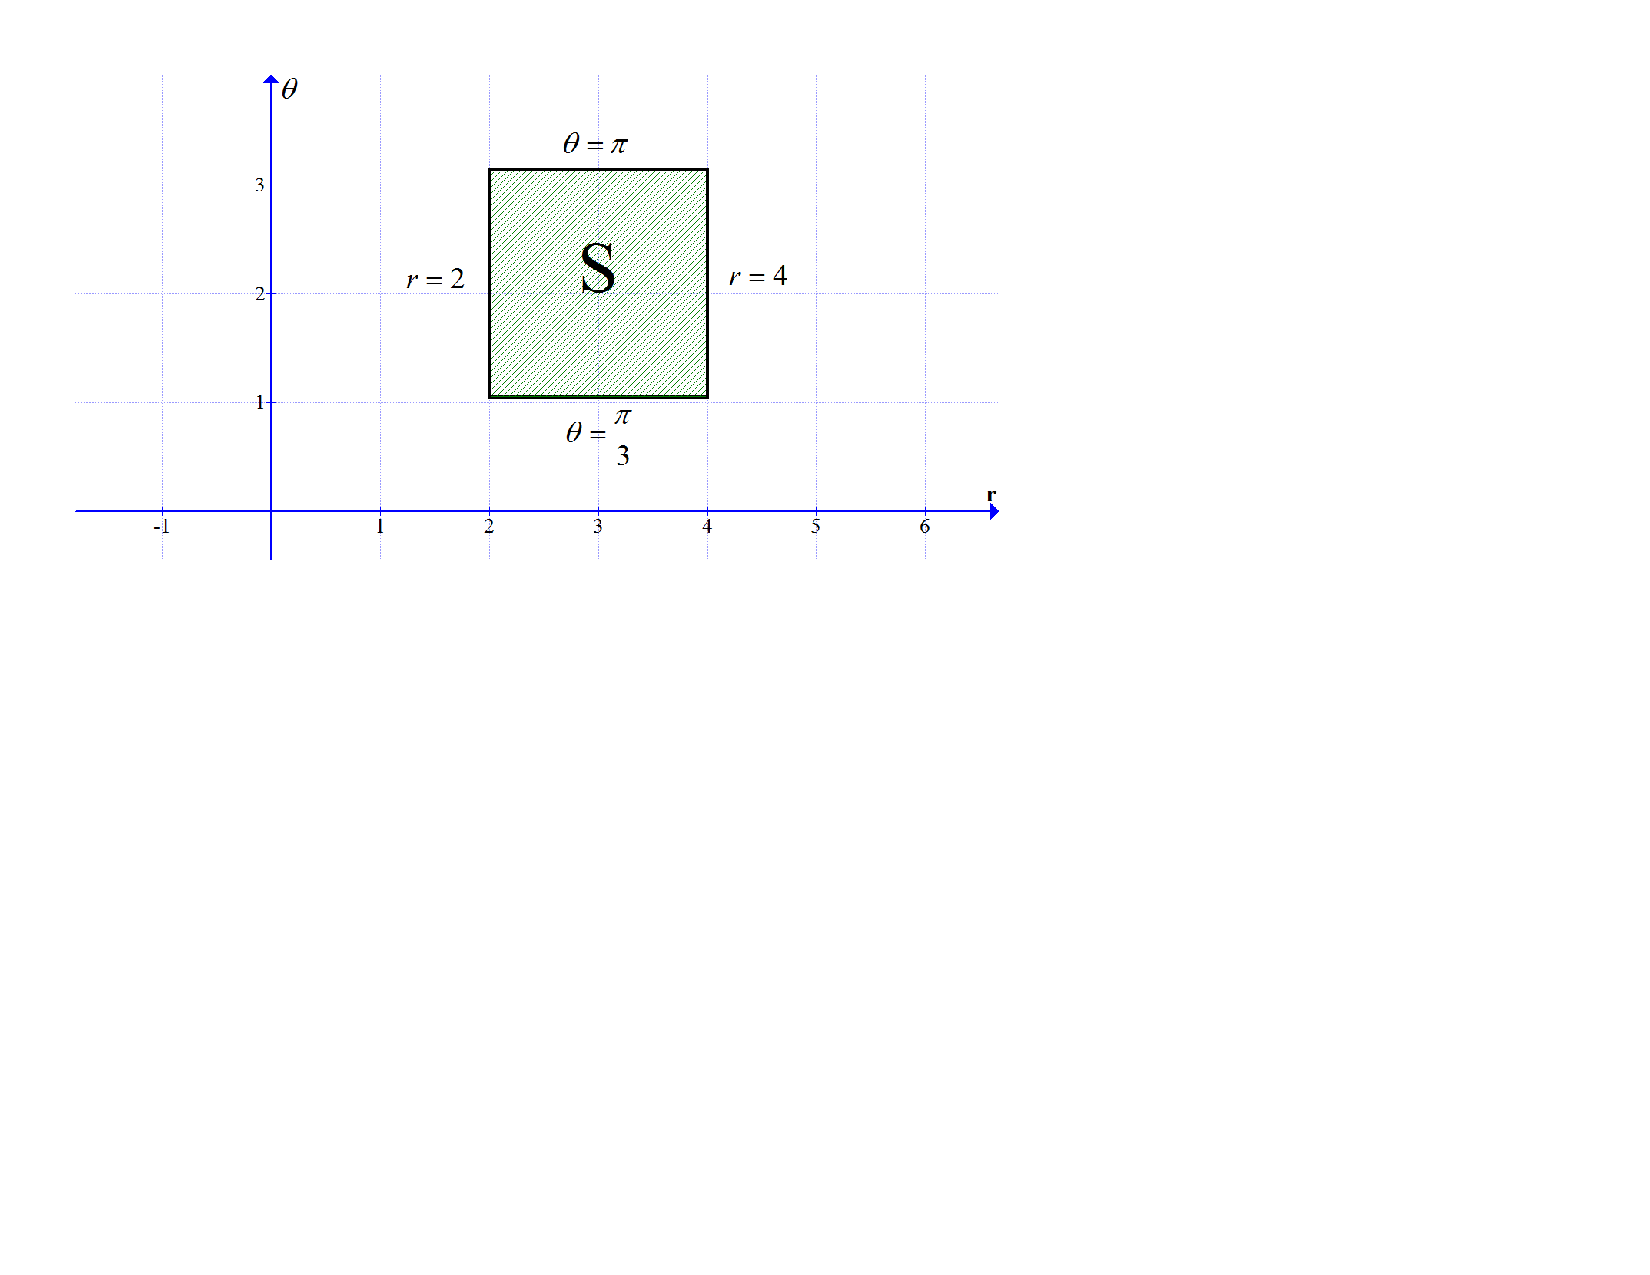
\includegraphics[scale=0.5]{region1a.pdf}}} \fi

\newpage

\item $R$ is the region shown below and the transformation is: $x=2u+v$, $y=2u+2v$.

\begin{center}
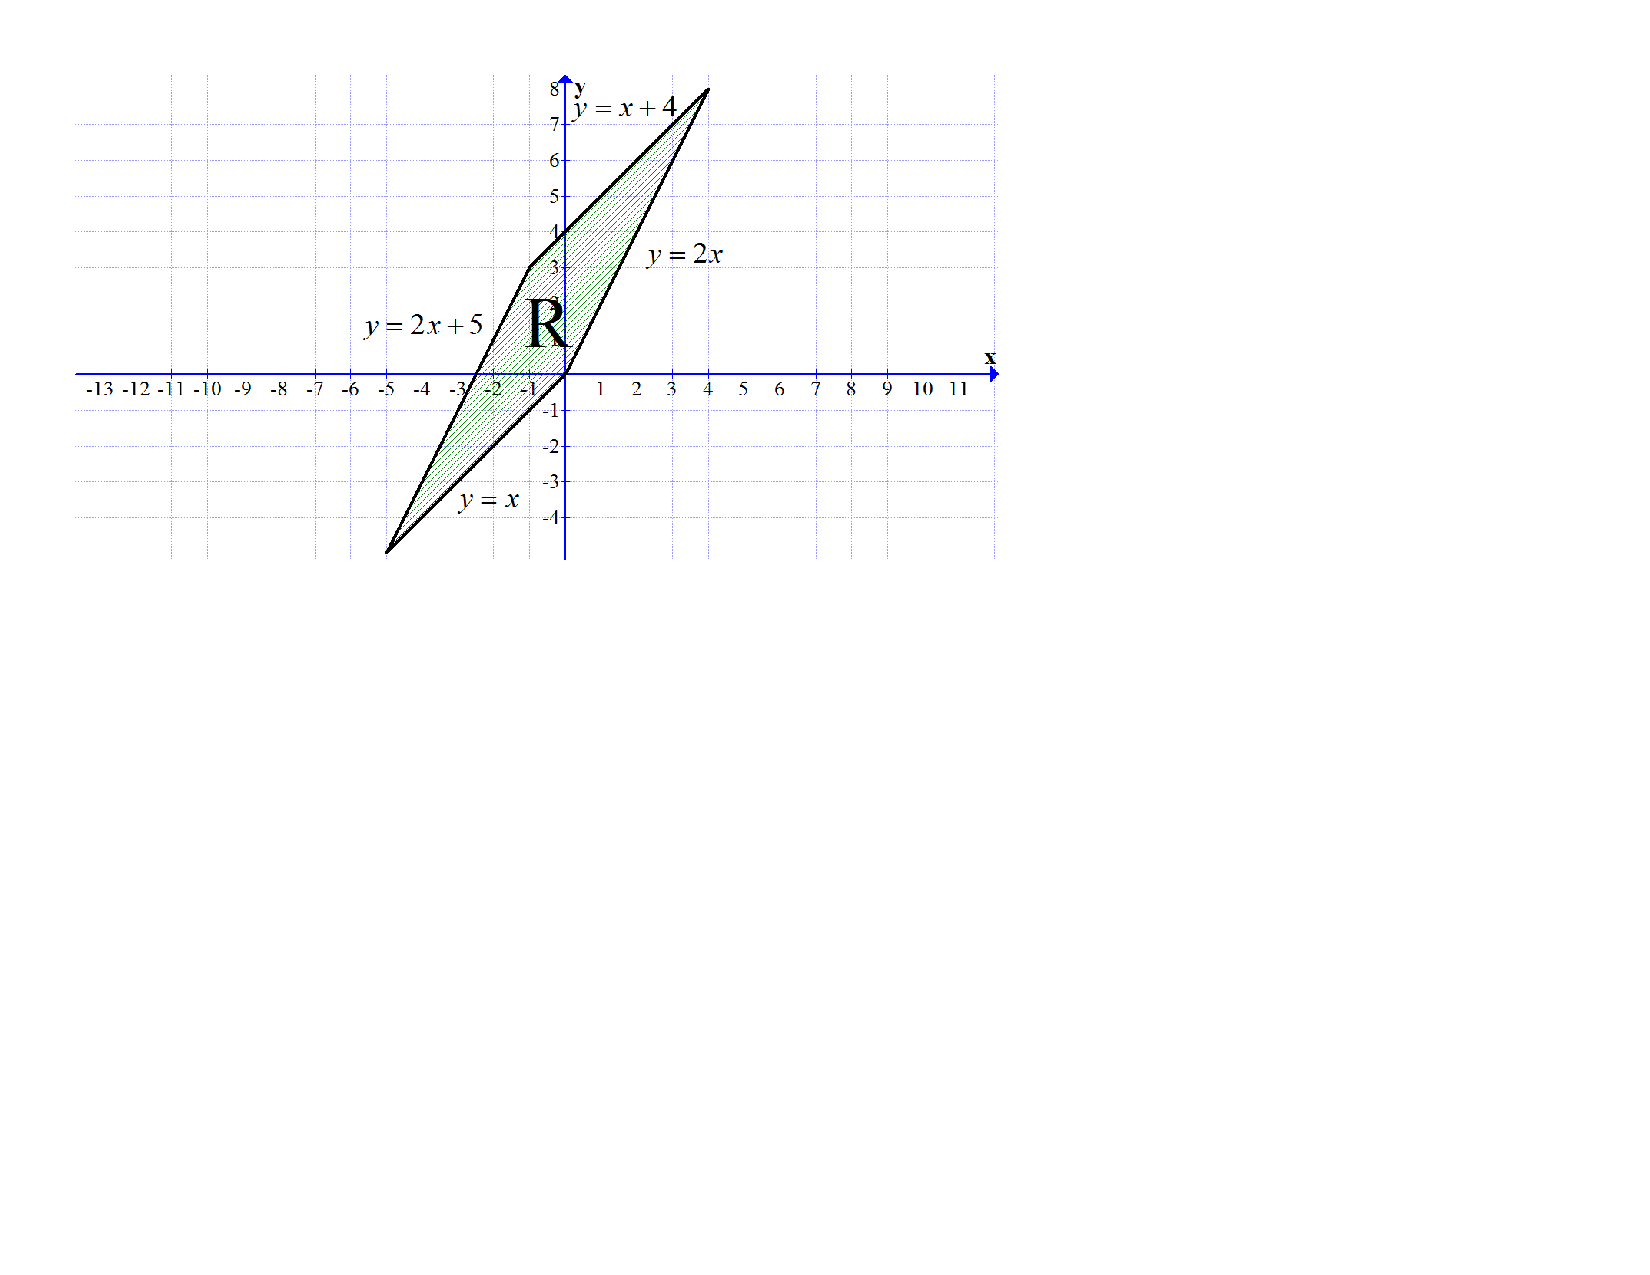
\includegraphics[scale=0.6]{region2.pdf}
\end{center}

\ifans{\fbox{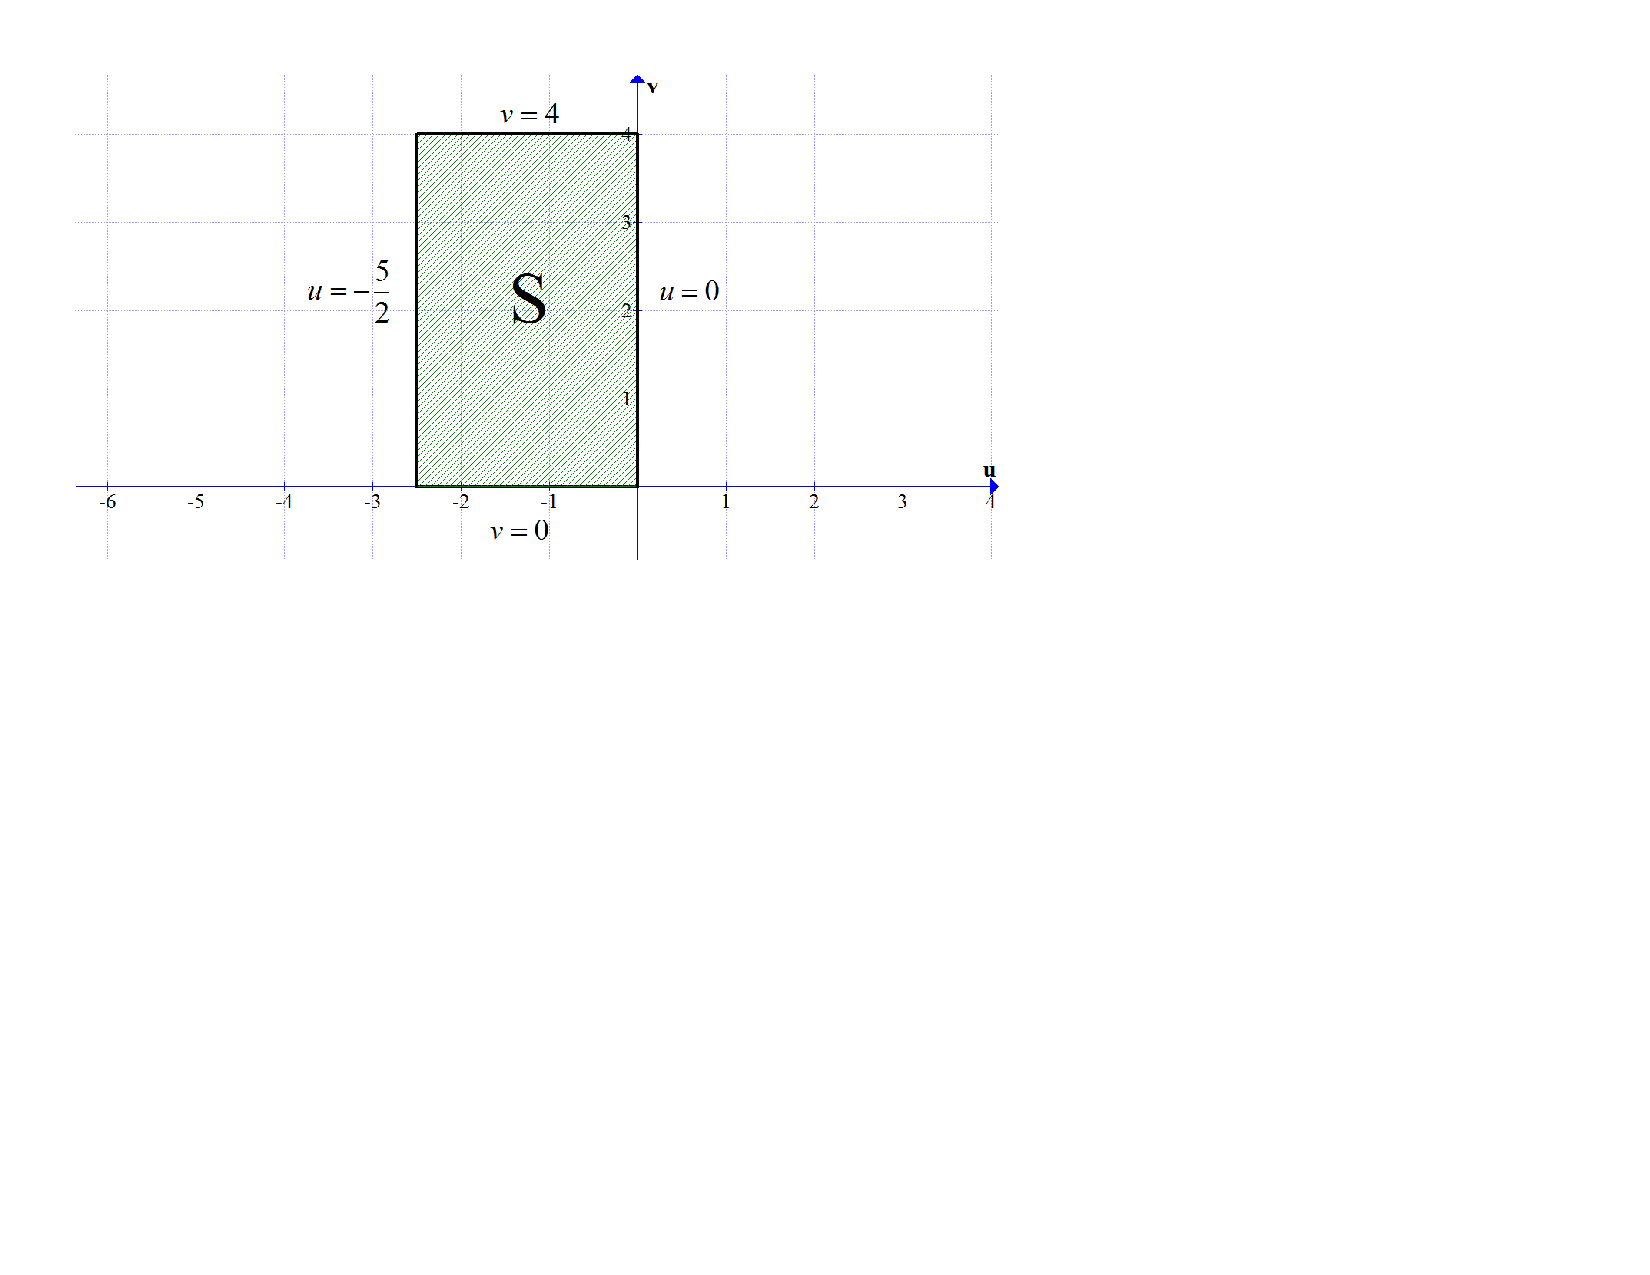
\includegraphics[scale=0.5]{region2a.pdf}}} \fi

\end{enumerate}

\item Consider the region $R$ shown below in the $xy$-plane.

\begin{center}
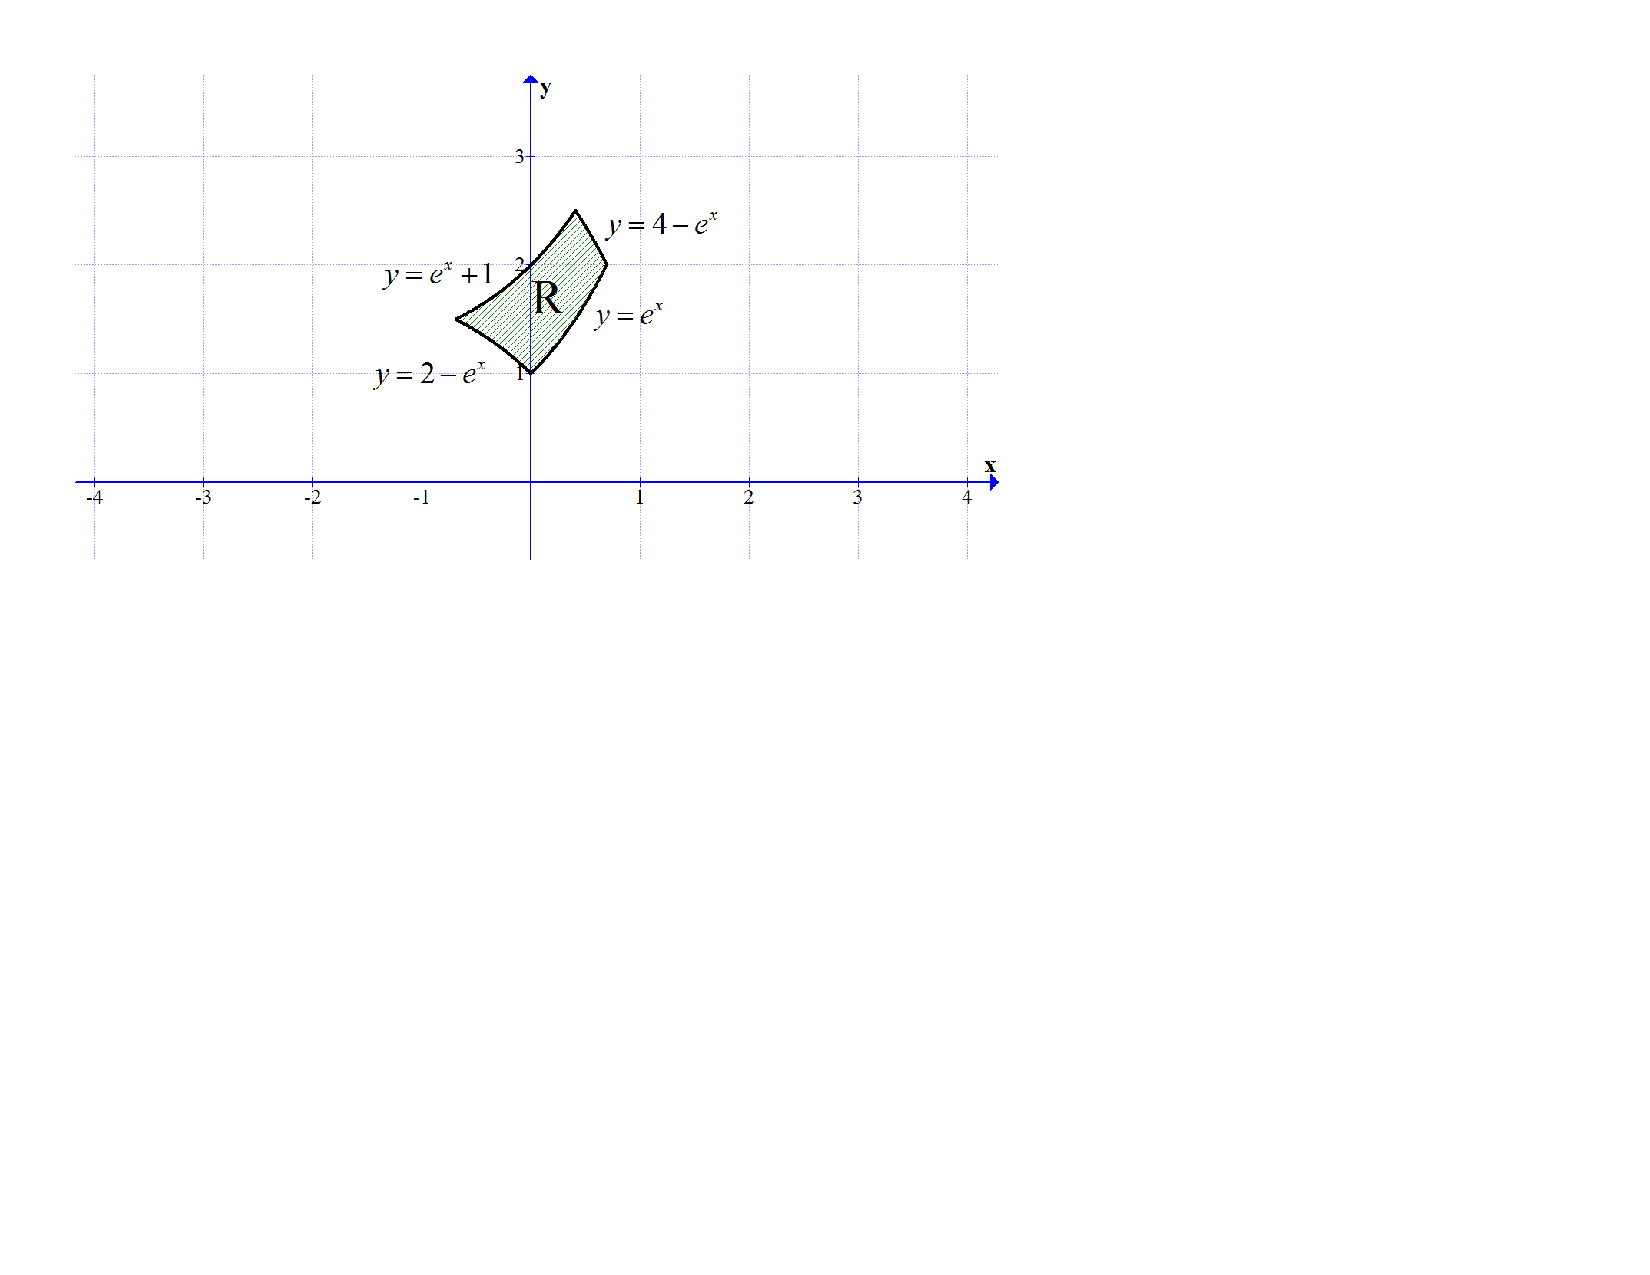
\includegraphics[scale=0.7]{region3.pdf}
\end{center}

\begin{enumerate}

\item Find a transformation that would map a rectangular region $S$ in the $uv$ plane to the region $R$ in the $xy$ plane.  (You may express your answer as $u=u(x,y)$ and $v=v(x,y)$.)

\ifans{\fbox{$u=y-e^x$, $v=y+e^x$}} \fi

\item Sketch the region $S$ from part (a) whose image under your transformation is $R$.

\ifans{\fbox{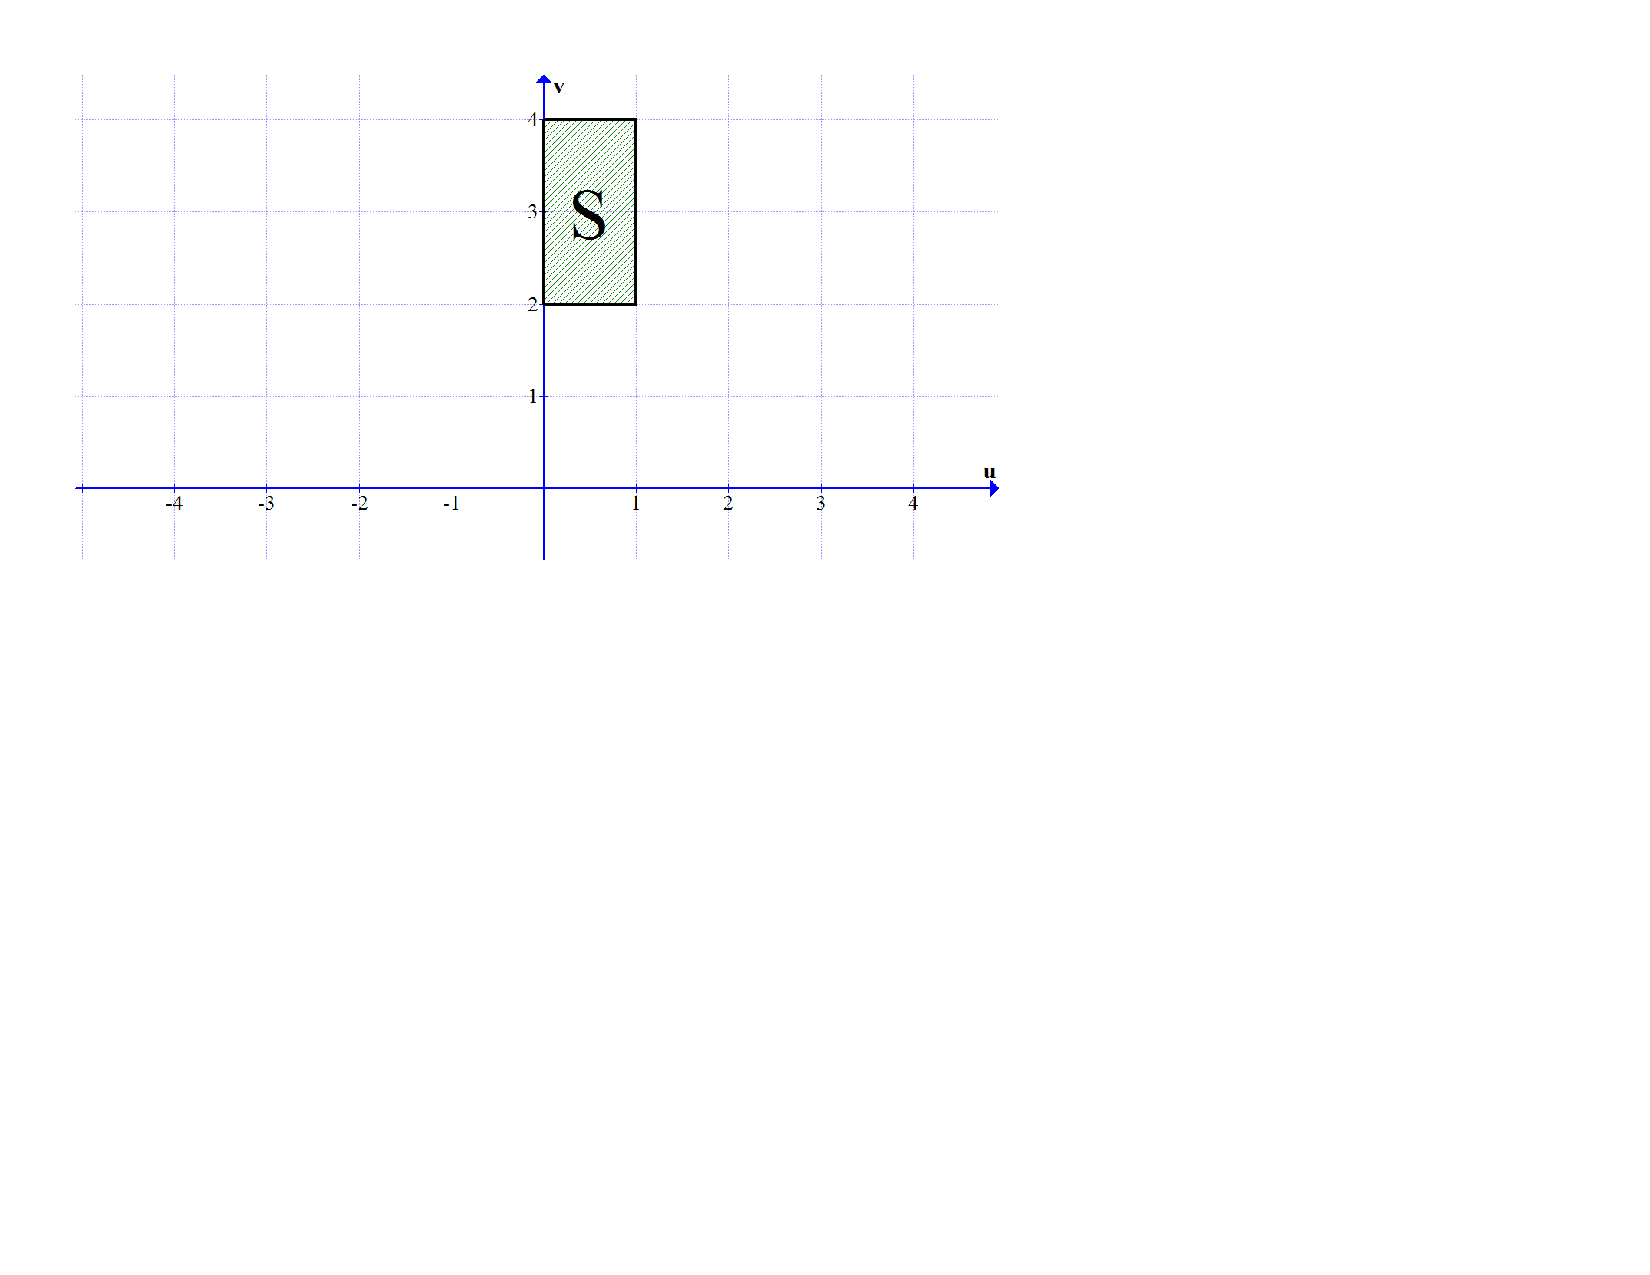
\includegraphics[scale=0.5]{region3s.pdf}}} \fi

\item Solve for $x$ and $y$ in terms of $u$ and $v$.  In doing so, you are finding the inverse transformation.  (You may express your answer as $x=x(u,v)$, $y=y(u,v)$.)

\ifans{\fbox{$x=\ln\left(\frac{1}{2}(v-u)\right)$ (where $v>u$), $y=\frac{1}{2}(u+v)$}} \fi

\end{enumerate}

\item For each of the following transformations, compute the Jacobian $\frac{\partial(x,y)}{\partial(u,v)}$.

\begin{enumerate}

\item $x=u+2v$, $y=-3u+v$

\ifans{\fbox{7}} \fi

\item $x=ve^u$, $y=ve^{-u}$

\ifans{\fbox{$2v$}} \fi

\item $x=e^{u}\cos{v}$ and $y=e^{u}\sin{v}$.  

\ifans{\fbox{$e^{2u}$}} \fi

\end{enumerate}

\item Consider the transformation $x=u+v$, $y=v-u$.

\begin{enumerate}

\item Compute the Jacobian $\frac{\partial(x,y)}{\partial(u,v)}$.

\ifans{\fbox{2}} \fi

\item Solve the $u$ and $v$ in terms of $x$ and $y$. (That is, find the inverse transformation.)

\ifans{\fbox{$u=\frac{1}{2}(x-y)$, $v=\frac{1}{2}(x+y)$}} \fi

\item Compute the Jacobian $\frac{\partial(u,v)}{\partial(x,y)}$ for the transformation that you found in part (b).

\ifans{\fbox{$\frac{1}{2}$}} \fi

\end{enumerate}

\item Verify that the Jacobian $\frac{\partial(x,y)}{\partial(r,\theta)}$ for the transformation $x=r\cos{\theta}$, $y=r\sin{\theta}$ is $r$.

\ifans{\fbox{$\frac{\partial(x,y)}{\partial(r,\theta)}=\begin{vmatrix}\cos{\theta} & -r\sin{\theta}\\ \sin{\theta} & r\cos{\theta}\end{vmatrix}=r\cos^2{\theta}+r\sin^2{\theta}=r$}} \fi

\item Verify that the Jacobian $\frac{\partial(x,y,z)}{\partial(\rho,\theta,\phi)}$ for the transformation $x=\rho\cos{\theta}\sin{\phi}$, $y=\rho\sin{\theta}\sin{\phi}$, $z=\rho\cos{\phi}$ is $\rho^2\sin{\phi}$.

\ifans{\fbox{$\frac{\partial(x,y,z)}{\partial(\rho,\theta,\phi)}=\begin{vmatrix} \cos{\theta}\sin{\phi} & -\rho\sin{\theta}\cos{\phi} & \rho\cos{\theta}\cos{\phi}\\ \sin{\theta}\sin{\phi} & \rho\cos{\theta}\sin{\phi} & \rho\sin{\theta}\cos{\phi}\\ \cos{\phi} & 0 & -\rho\sin{\phi} \end{vmatrix}=\dots = \rho^2\sin{\phi}$}} \fi

\item Use the transformation $u=3x+y$, $v=6x-y$ to evaluate $\iint \limits_{R} \frac{3x+y}{6x-y} \,dA$ where $R$ is the region enclosed by $3x+y=2$, $3x+y=-3$, $6x-y=1$, $6x-y=e$.

\ifans{\fbox{$-\frac{5}{18}$}} \fi

\item Use the transformation $u=x-y$, $v=x+y$ to evaluate $\iint \limits_{R} e^{(x-y)^2} \,dA$ where $R$ is the region in the $xy$ plane which is enclosed by $y=0$, $y=-x$, and $y=x-1$.

\ifans{\fbox{$\frac{1}{4}(e-1)$; Detailed Solution: \textcolor{blue}{\href{http://www.math.drexel.edu/classes/Calculus/resources/Math200HW/Solutions/21_200_COV_08.pdf}{Here}}}} \fi

\item Use the transformation $x=au$, $y=bv$, and $z=cw$ to evaluate $\displaystyle \iiint_{G}  \,\mathrm{d}V$, where $G = \displaystyle \big\{ (x,y,z) : \frac{x^2}{a^2}+\frac{y^2}{b^2}+\frac{z^2}{c^2}\leq 1 \big\}$.  Note: $a$, $b$ and $c$ are real, positive constants.

\ifans{\fbox{$\frac{4\pi}{3}abc$; This is the volume of the ellipsoid  $\frac{x^2}{a^2}+\frac{y^2}{b^2}+\frac{z^2}{c^2} = 1$}} \fi

\newpage

\item Use the transformation $u=2x+y$, $v=-2x+y$ to compute the area of the region $R$, shown below.

\begin{center}
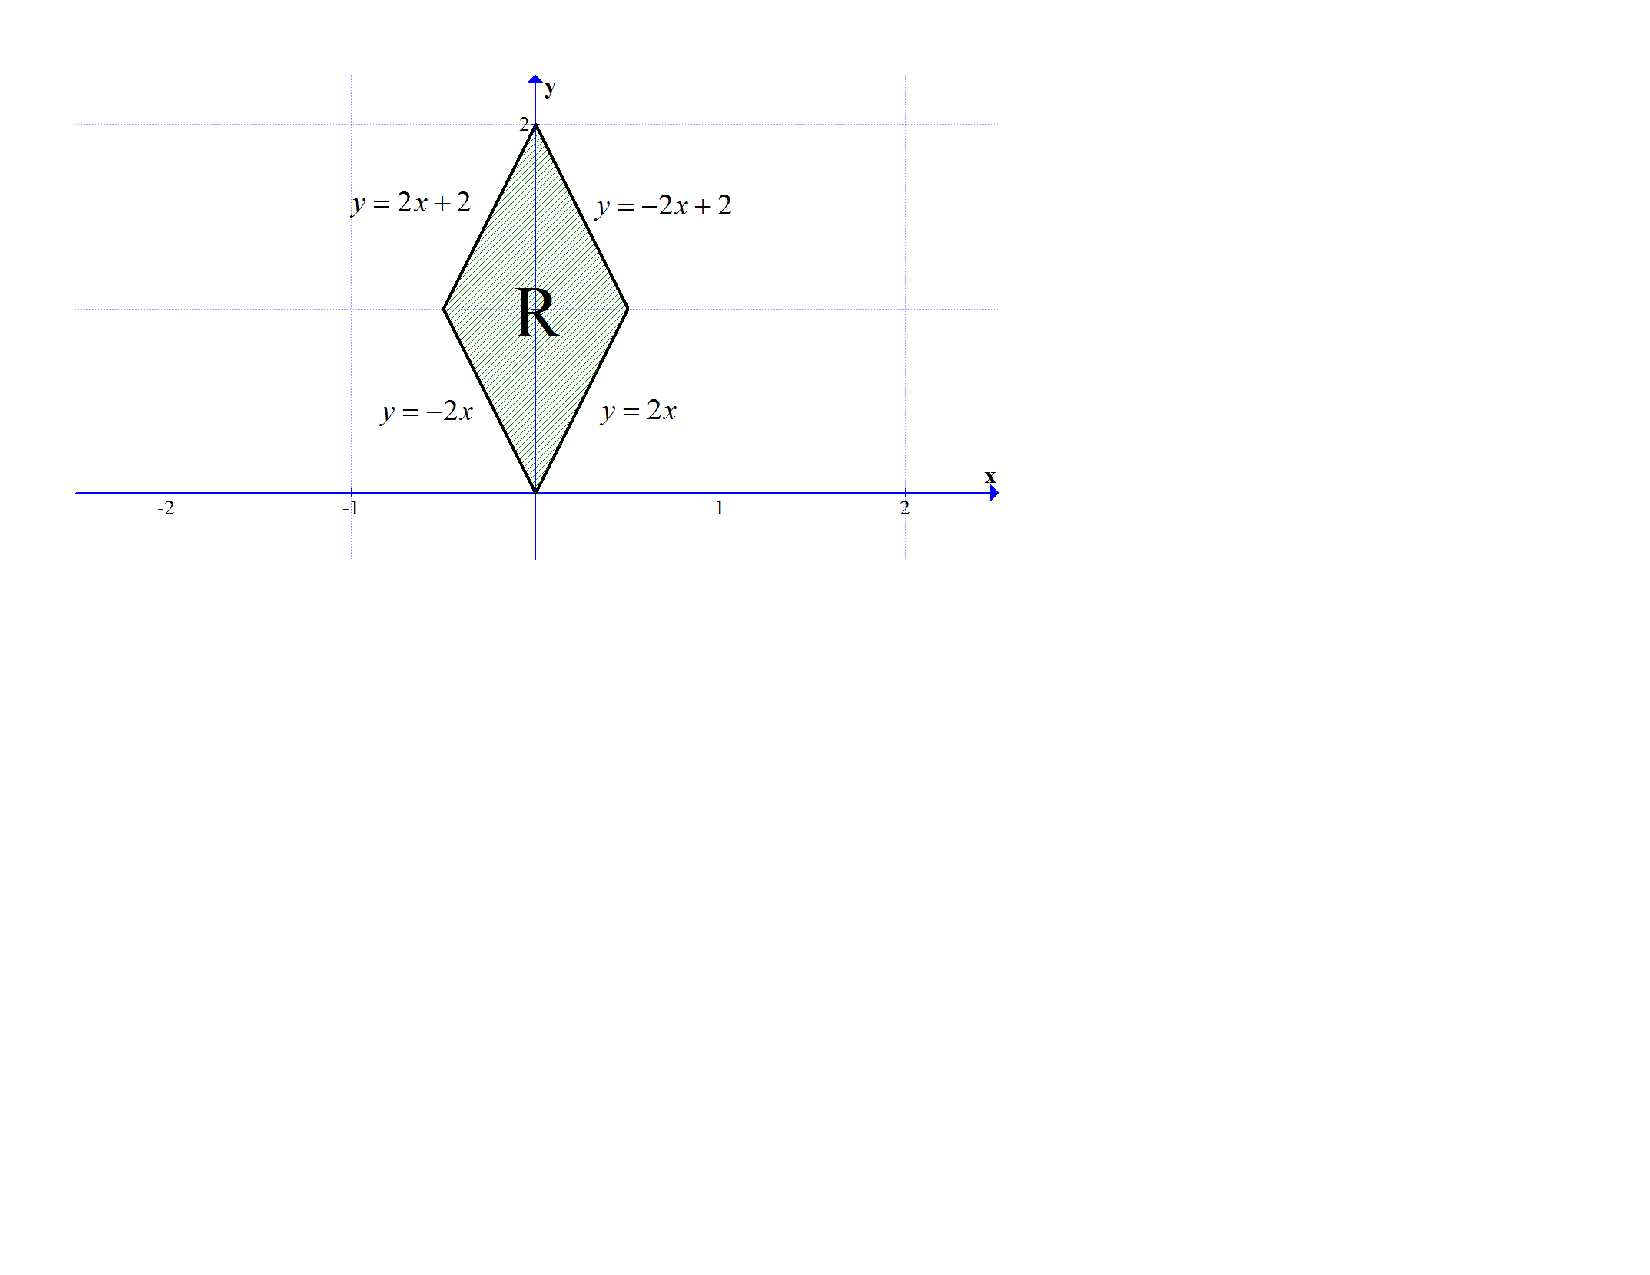
\includegraphics[scale=0.6]{region4.pdf}
\end{center}

\ifans{\fbox{1}} \fi

\item Compute the area of the region $R$ described in exercise 2.

\ifans{\fbox{$6\ln{2}-3\ln{3}$}} \fi

\end{enumerate}

\end{document}